\documentclass[12pt]{report}
\usepackage[utf8]{inputenc}
\usepackage[russian]{babel}
%\usepackage[14pt]{extsizes}
\usepackage{listings}
\usepackage{graphicx}
\usepackage{amsmath,amsfonts,amssymb,amsthm,mathtools} 
\usepackage{pgfplots}
\usepackage{filecontents}
\usepackage{indentfirst}
\usepackage{eucal}
\usepackage{amsmath}
\usepackage{enumitem}
\frenchspacing

\usepackage{indentfirst} % Красная строка


%\usetikzlibrary{datavisualization}
%\usetikzlibrary{datavisualization.formats.functions}

\usepackage{amsmath}


% Для листинга кода:
\lstset{ %
language=caml,                 % выбор языка для подсветки (здесь это С)
basicstyle=\small\sffamily, % размер и начертание шрифта для подсветки кода
numbers=left,               % где поставить нумерацию строк (слева\справа)
numberstyle=\tiny,           % размер шрифта для номеров строк
stepnumber=1,                   % размер шага между двумя номерами строк
numbersep=5pt,                % как далеко отстоят номера строк от подсвечиваемого кода
showspaces=false,            % показывать или нет пробелы специальными отступами
showstringspaces=false,      % показывать или нет пробелы в строках
showtabs=false,             % показывать или нет табуляцию в строках
frame=single,              % рисовать рамку вокруг кода
tabsize=2,                 % размер табуляции по умолчанию равен 2 пробелам
captionpos=t,              % позиция заголовка вверху [t] или внизу [b] 
breaklines=true,           % автоматически переносить строки (да\нет)
breakatwhitespace=false, % переносить строки только если есть пробел
escapeinside={\#*}{*)}   % если нужно добавить комментарии в коде
}

\usepackage[left=2cm,right=2cm, top=2cm,bottom=2cm,bindingoffset=0cm]{geometry}
% Для измененных титулов глав:
\usepackage{titlesec, blindtext, color} % подключаем нужные пакеты
\definecolor{gray75}{gray}{0.75} % определяем цвет
\newcommand{\hsp}{\hspace{20pt}} % длина линии в 20pt
% titleformat определяет стиль
\titleformat{\chapter}[hang]{\Huge\bfseries}{\thechapter\hsp\textcolor{gray75}{|}\hsp}{0pt}{\Huge\bfseries}


% plot
\usepackage{pgfplots}
\usepackage{filecontents}
\usetikzlibrary{datavisualization}
\usetikzlibrary{datavisualization.formats.functions}

\begin{document}
%\def\chaptername{} % убирает "Глава"
\thispagestyle{empty}
\begin{titlepage}
	\noindent \begin{minipage}{0.15\textwidth}
	
\includegraphics[width=\linewidth]{b_logo}
	\end{minipage}
	\noindent\begin{minipage}{0.9\textwidth}\centering
		\textbf{Министерство науки и высшего образования Российской Федерации}\\
		\textbf{Федеральное государственное бюджетное образовательное учреждение высшего образования}\\
		\textbf{~~~«Московский государственный технический университет имени Н.Э.~Баумана}\\
		\textbf{(национальный исследовательский университет)»}\\
		\textbf{(МГТУ им. Н.Э.~Баумана)}
	\end{minipage}
	
	\noindent\rule{18cm}{3pt}
	\newline\newline
	\noindent ФАКУЛЬТЕТ $\underline{\text{«Информатика и системы управления»}}$ \newline\newline
	\noindent КАФЕДРА $\underline{\text{«Программное обеспечение ЭВМ и информационные технологии»}}$\newline\newline\newline\newline\newline
	
	
	\begin{center}
		\noindent\begin{minipage}{1.3\textwidth}\centering
			\Large\textbf{  Отчёт по лабораторной работе №3}\newline
			\textbf{по дисциплине "Анализ алгоритмов"}\newline\newline
		\end{minipage}
	\end{center}
	
	\noindent\textbf{Тема} $\underline{\text{Алгоритмы сортировки}}$\newline\newline
	\noindent\textbf{Студент} $\underline{\text{Романов А.В.}}$\newline\newline
	\noindent\textbf{Группа} $\underline{\text{ИУ7-53Б}}$\newline\newline
	\noindent\textbf{Оценка (баллы)} $\underline{\text{~~~~~~~~~~~~~~~~~~~~~~~~~~~}}$\newline\newline
	\noindent\textbf{Преподаватели} $\underline{\text{Волкова Л.Л., Строганов Ю.В.}}$\newline\newline\newline
	
	\begin{center}
		\vfill
		Москва~---~\the\year
		~г.
	\end{center}
\end{titlepage}


\tableofcontents

\newpage
\chapter*{Введение}
\addcontentsline{toc}{chapter}{Введение}


Одной из важнейших процедур обработки структурированной информации является сортировка. Сортировкой называют процесс перегруппировки заданной последовательности (кортежа) объектов в некотором определенном порядке. Определенный порядок (например, упорядочение в алфавитном порядке, по возрастанию или убыванию количественных характеристик, по классам, типам и.т.п.) в последовательности объектов необходимо для удобства работы с этим объектом . В частности, одной из целей сортировки является облегчение последующего поиска элементов в отсортированном множестве. 

Алгоритмы сортировки используются практически в любой программной системе. Целью алгоритмов сортировки является упорядочение последовательности элементов данных. Поиск элемента в последовательности отсортированных данных занимает время, пропорциональное логарифму количеству элементов в последовательности, а поиск элемента в последовательности не отсортированных данных занимает время, пропорциональное количеству элементов в последовательности, то есть намного больше. Существует множество различных методов сортировки данных. Однако любой алгоритм сортировки можно разбить на три основные части:

\begin{itemize}
	\item сравнение, определяющее упорядоченность пары элементов;
	\item перестановка, меняющая местами пару элементов;
	\item сортирующий алгоритм, который осуществляет сравнение и перестановку элементов данных до тех пор, пока все эти элементы не будут упорядочены.
\end{itemize}

Важнейшей характеристикой любого алгоритма сортировки является скорость его работы, которая определяется функциональной зависимостью среднего времени сортировки последовательностей элементов данных, заданной длины, от этой длины. Время сортировки будет пропорционально количеству сравнений и перестановки элементов данных в процессе их сортировки. Как уже было сказано, в любой сфере, использующей какое-либо программное обеспечение, с большой долей вероятности используются сортировки.  

""\newline
Задачи лабораторной работы:
\begin{itemize}
	\item изучить и реализовать 3 алгоритма сортировки: пузырёк, вставками, быстрая сортировка;
	\item провести сравнительный анализ трудоёмкости алгоритмов на основе теоретических расчетов и выбранной модели вычислений;
	\item провести сравнительный анализ алгоритмов на основе экспериментальных данных.
\end{itemize}

\chapter{Аналитическая часть}

\section{Сортировка пузырьком}

Алгоритм состоит из повторяющихся проходов по сортируемому массиву.
За каждый проход элементы последовательно сравниваются попарно и, если порядок в паре неверный, выполняется обмен элементов.
Проходы по массиву повторяются $N-1$ раз, но есть модифицированная версия, где если окажется, что обмены больше не нужны, значит проходы прекращаются.
При каждом проходе алгоритма по внутреннему циклу очередной наибольший элемент массива ставится на свое место в конце массива рядом с предыдущим ``наибольшим элементом'', а наименьший элемент массива перемещается на одну позицию к началу массива (``всплывает'' до нужной позиции, как пузырёк в воде -- отсюда и название алгоритма).

\section{Сортировка вставками}

Сортировка вставками — алгоритм сортировки, котором элементы входной последовательности просматриваются по одному, и каждый новый поступивший элемент размещается в подходящее место среди ранее упорядоченных элементов.

В начальный момент отсортированная последовательность пуста.
На каждом шаге алгоритма выбирается один из элементов входных данных и помещается на нужную позицию в уже отсортированной последовательности до тех пор, пока набор входных данных не будет исчерпан.
В любой момент времени в отсортированной последовательности элементы удовлетворяют требованиям к выходным данным алгоритма.

\section{Быстрая сортировка}

Общая идея алгоритма состоит в следующем:

\begin{enumerate}
	\item выбрать из массива элемент, называемый опорным. Это может быть любой из элементов массива. От выбора опорного элемента не зависит корректность алгоритма, но в отдельных случаях может сильно зависеть его эффективность 
	\item сравнить все остальные элементы с опорным и переставить их в массиве так, чтобы разбить массив на три непрерывных отрезка, следующих друг за другом: «элементы меньшие опорного», «равные» и «большие».
	\item для отрезков «меньших» и «больших» значений выполнить рекурсивно ту же последовательность операций, если длина отрезка больше единицы.
\end{enumerate}

На практике массив обычно делят не на три, а на две части: например, «меньшие опорного» и «равные и большие»; такой подход в общем случае эффективнее, так как упрощает алгоритм разделения 

\section{Вывод}

В данном разделе были рассмотрены 3 алгоритмы сортировки: пузырьком, вставками и быстрая сортировка.
	
\clearpage

\chapter{Конструкторская часть}

\section{Схемы алгоритмов}

На рисунках 2.1, 2.2 и 2.3 показаны схемы алгоритмов сортировки пузырьком, вставками и быстрой сортировки соответственно.

\begin{figure}[h]
	\centering
	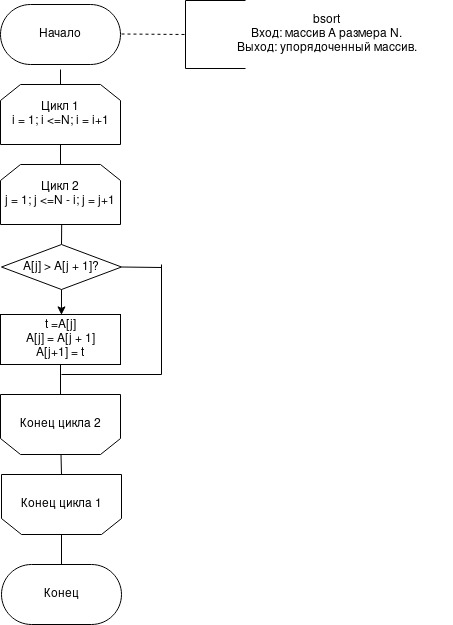
\includegraphics[width=0.9\linewidth]{bsort.jpg}
	\caption{Схема сортировки пузырьком}
	\label{fig:mpr}
\end{figure}

\begin{figure}[h]
	\centering
	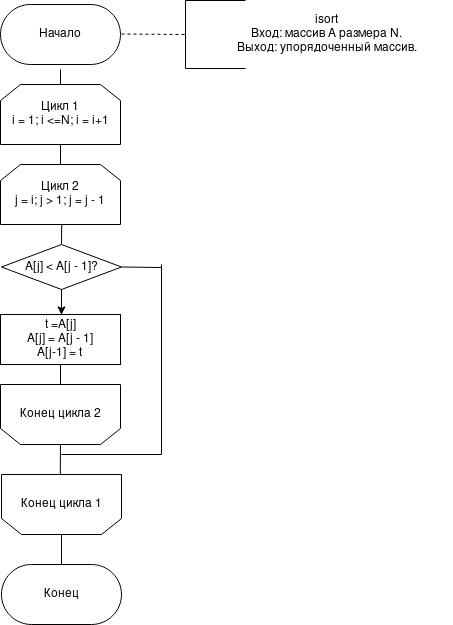
\includegraphics[width=0.9\linewidth]{isort.jpg}
	\caption{Схема сортировки вставками}
	\label{fig:mpr}
\end{figure}

\begin{figure}[h]
	\centering
	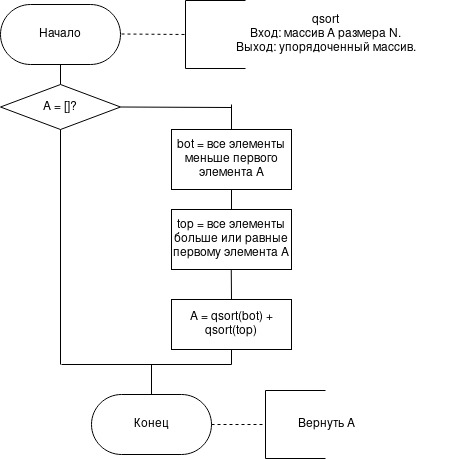
\includegraphics[width=1\linewidth]{qsort.jpg}
	\caption{Схема быстрой сортировки}
	\label{fig:mpr}
\end{figure}


\section{Модель вычислений}

Для последующего вычисления трудоемкости введём модель вычислений:

\begin{enumerate}
	\item Операции из списка (\ref{for:opers}) имеют трудоемкость 1.
	\begin{equation}
	\label{for:opers}
	+, -, /, \%, ==, !=, <, >, <=, >=, [], ++, {-}-
	\end{equation}
	\item Трудоемкость оператора выбора if условие then A else B рассчитывается, как (\ref{for:if}).
	\begin{equation}
	\label{for:if}
	f_{if} = f_{\text{условия}} +
	\begin{cases}
	f_A, & \text{если условие выполняется,}\\
	f_B, & \text{иначе.}
	\end{cases}
	\end{equation}
	\item Трудоемкость цикла рассчитывается, как (\ref{for:for}).
	\begin{equation}
	\label{for:for}
	f_{for} = f_{\text{инициализации}} + f_{\text{сравнения}} + N(f_{\text{тела}} + f_{\text{инкремента}} + f_{\text{сравнения}})
	\end{equation}
	\item Трудоемкость вызова функции равна 0.
\end{enumerate}

\section{Трудоёмкость алгоритмов}

Пусть размер массивов во всех вычислениях обозначается как $N$.

\subsection{Алгоритм сортировки пузырьком}

Трудоёмкость алгоритма сортировки пузырьком состоит из:
\begin{itemize}
	\item трудоёмкость сравнения и инкремента внешнего цикла $i \in [1..N)$ (\ref{for:bubble_outer}):
	\begin{equation}
	\label{for:bubble_outer}
	f_{i} = 2 + 2(N - 1)
	\end{equation}
	\item суммарная трудоёмкость внутренних циклов, количество итераций которых меняется в промежутке $[1..N-1]$ (\ref{for:bubble_inner}):
	\begin{equation}
	\label{for:bubble_inner}
	f_{j} = 3(N - 1) + \frac{N \cdot (N - 1)}{2} \cdot (3 + f_{if})
	\end{equation}
	\item трудоёмкость условия во внутреннем цикле (\ref{for:bubble_if}):
	\begin{equation}
	\label{for:bubble_if}
	f_{if} = 4 + \begin{cases}
	0, & \text{в лучшем случае}\\
	9, & \text{в худшем случае}\\
	\end{cases}
	\end{equation}
\end{itemize}

Трудоёмкость в \textbf{лучшем} случае (\ref{for:bubble_best}):
\begin{equation}
\label{for:bubble_best}
f_{best} = \frac{7}{2} N^2 + \frac{3}{2} N - 3 \approx \frac{7}{2} N^2 = O(N^2)
\end{equation}

Трудоёмкость в \textbf{худшем} случае (\ref{for:bubble_worst}):
\begin{equation}
\label{for:bubble_worst}
f_{worst} =  8N^2 - 8N - 3 \approx 8N^2 = O(N^2)
\end{equation}

\subsection{Алгоритм сортировки вставками}

Трудоёмкость алгоритма сортировки пузырьком состоит из:
\begin{itemize}
	\item трудоёмкость сравнения и инкремента внешнего цикла $i \in [1..N)$ (\ref{for:isort_outer}):
	\begin{equation}
	\label{for:isort_outer}
	f_{i} = 2 + 2(N - 1)
	\end{equation}
	\item суммарная трудоёмкость внутренних циклов, количество итераций которых меняется в промежутке $[1..N-1]$ (\ref{for:isort_inner}):

	\begin{equation}
	\label{for:isort_inner}
	f_{if} = 4 + \begin{cases}
		0, & \text{в лучшем случае}\\
		3(N - 1) + \frac{N \cdot (N - 1)}{2} \cdot (3 + f_{if}), & \text{в худшем случае}\\
	\end{cases}
	\end{equation}

	\item трудоёмкость условия во внутреннем цикле (\ref{for:isort_if}):
	\begin{equation}
	\label{for:isort_if}
	f_{if} = 4 + \begin{cases}
	0, & \text{в лучшем случае}\\
	9, & \text{в худшем случае}\\
	\end{cases}
	\end{equation}
\end{itemize}

Трудоёмкость в \textbf{лучшем} случае (\ref{for:isort_best}):
\begin{equation}
\label{for:isort_best}
f_{best} = 13N - 10 \approx 13N = O(N)
\end{equation}

Трудоёмкость в \textbf{худшем} случае (\ref{for:isort_worst}):
\begin{equation}
\label{for:isort_worst}
f_{worst} = 4.5N^2 + 10N - 13 \approx 4N^2 = O(N^{2})
\end{equation}

\section{Вывод}

На основе теоретических данных, полученных из аналитического раздела, были построены схемы трёх алгоритмов сортировки. Оценены их тредёмкости в лучшем и худшем случаях.

\chapter{Технологическая часть}

В данном разделе приведены средства реализации и листинги кода.

\section{Требование к ПО}

К программе предъявляется ряд требований:

\begin{itemize}
	\item на вход ПО получает массив сравнимых элементов;
	\item на выходе -- тот же массив, но отсортированный в заданном порядке.
\end{itemize}

\section{Средства реализации}
Для реализации ПО я выбрал язык программирования OCaml \cite{Ocaml}. Данный выбор обусловлен моим желанием расширить свои знания в области применения данного язкыа программирования. 

\section{Реализация алгоритмов}

В листингах 3.1 - 3.3 приведена реализация трёх алгоритмов сортировки.

\begin{lstlisting}[label=some-code,caption=Функция сортировки массива пузырьком, language=Caml]
let rec bsort arr =
  let rec _bsort = function
    | x1 :: x2 :: xs when x1 > x2 -> x2 :: _bsort (x1 :: xs)
    | x1 :: x2 :: xs -> x1 :: _bsort (x2 :: xs)
    | arr -> arr
  in
  let maybe_sorted = _bsort arr in
    if maybe_sorted = arr then arr
  else bsort maybe_sorted
;;
\end{lstlisting}

\begin{lstlisting}[label=some-code,caption=Функция сортировки массива вставками,language=Caml]
let rec isort arr =
  let rec insert k = function
    | x :: xs when k < x -> k :: x :: xs
    | x :: xs -> x :: (insert k xs)
    | arr -> [k]
  in
    match arr with
    | [] -> []
    | x :: xs -> insert x (isort xs)
;;
\end{lstlisting}

\begin{lstlisting}[label=some-code,caption=Функция быстрой сортировки,language=Caml]
let rec qsort = function
    | [] -> []
    | x :: xs -> let bot, top = List.partition (fun a -> a < x) xs
                 in qsort bot @ (x :: qsort top)
;;
\end{lstlisting}

\section{Тестовые данные}

В таблице~\ref{tbl:test} приведены тесты для функций, реализующих алгоритмы сортировки. Все тесты пройдены успешно.

\begin{table}[h!]
	\begin{center}
		\begin{tabular}{|c|c|c|}
			\hline
			Входной массив & Результат & Ожидаемый результат \\ 
			\hline
			$[15, 25, 35, 45, 55]$ & $[15, 25, 35, 45, 55]$  & $[15, 25, 35, 45, 55]$\\\hline
			$[55, 45, 35, 25, 15]$  & $[15, 25, 35, 45, 55]$ & $[15, 25, 35, 45, 55]$\\\hline
			$[-10, -20, -30, -25, -50]$  & $[-50, -30, -25, -20, -10]$  & $[-50, -30, -25, -20, -10]$\\\hline
			$[40, -10, 20, -30, 75]$  & $[-30, -10, 20, 40, 75]$  & $[-30, -10, 20, 40, 75]$\\\hline
			$[100]$  & $[100]$  & $[100]$\\\hline
			$[-20]$  & $[-20]$  & $[-20]$\\\hline
			Пустой массив  & Пустой массив  & Пустой массив\\
			\hline
		\end{tabular}
		\caption{\label{tbl:test}Тестирование функций}
	\end{center}
\end{table}

\section{Вывод}

В данном разделе были разработаны исходные коды трёх алгоритмов сортировки: пузырьком, вставками и быстрая сортировка.

\chapter{Исследовательская часть}

\section{Технические характеристики}

Ниже приведены технические характеристики устройства, на котором было проведено тестирование ПО:

\begin{itemize}
	\item Операционная система: Debian \cite{debian} Linux \cite{linux} 11 <<bullseye>> 64-bit.
	\item Оперативная память: 12 GB.
	\item Процессор: Intel(R) Core(TM) i5-3550 CPU @ 3.30GHz
\cite{i5}.

\end{itemize}

\section{Время выполнения алгоритмов}
Время выполнения алгоритм замерялось с помощью применения технологии профайлинга \cite{profiling}. Данный инстрмуент даёт детальное описание количества вызовов и количества времени CPU, занятого каждой функцией. \newline

\begin{table} [h!]
	\caption{Таблица времени выполнения сортировок на отсортированных данных (в секундах)}
	\begin{center}
	\begin{tabular}{|c c c c|}

		\hline

		Размер & bsort & isort & qsort  \\ [0.5ex]

		1000 & 0.01922 & 2e-05 & 0.00025 \\ 


		\hline 

		1200 & 0.02419 & 7e-05 & 0.00029 \\ 

		\hline 

		1400 & 0.03516 & 6e-05 & 0.00035 \\ 

		\hline 

		1600 & 0.04540 & 0.0001& 0.00034 \\ 

		\hline 

		1800 & 0.06051 & 6e-05 & 0.00032 \\ 

		\hline 

		2000 & 0.06591 & 9e-05 & 0.00038 \\ 

	\hline 

	\end{tabular}
	\end{center}
\end{table}

\begin{table} [h!]
	\caption{Таблица времени выполнения сортировок на отсортированных данных в обратном порядке (в секундах)}
	\begin{center}
	\begin{tabular}{|c c c c|}

		\hline

		Размер & bsort & isort & qsort \\ [0.5ex]

		1000 & 0.02464 & 0.02351 & 0.05463 \\ 

		\hline 
 

		1200 & 0.03504 & 0.03444 & 0.08216 \\ 

		\hline 

		1400 & 0.04539 & 0.04633 & 0.11752 \\ 

		\hline 

		1600 & 0.07741 & 0.06945 & 0.18477 \\ 

		\hline 

		1800 & 0.08010 & 0.07510 & 0.19965 \\ 

		\hline 

		2000 & 0.08919 & 0.08319 & 0.22478 \\ 

		\hline 

	\end{tabular}
	\end{center}
\end{table}

\begin{table} [h!]
	\caption{Таблица времени выполнения сортировок на случайных данных (в секундах)}
	\begin{center}
	\begin{tabular}{|c c c c|}

		\hline

		Размер & bsort & isort  & qsort \\ [0.5ex]

		1000 & 0.01937 & 0.01129 & 0.00065 \\ 

		\hline 

		1200 & 0.02371 & 0.01426 & 0.00042 \\ 

		\hline 

		1400 & 0.03296 & 0.01619 & 0.00095 \\ 

		\hline 

		1600 & 0.04761 & 0.01842 & 0.00143 \\ 

		\hline 

		1800 & 0.06122 & 0.02028 & 0.00145 \\ 

		\hline 

		2000 & 0.06756 & 0.02129 & 0.00220 \\ 

		\hline 

	\end{tabular}
	\end{center}
\end{table}

\section{Вывод}

Как и ожидалось в результате оценки трудоемкости алгоритмов, сортировка вставками работает очень быстро на уже отсортированном массиве. Время сортировки вставками на всех трёх видах массивов примерно одинаково.
При обратно отсортированном массиве, быстрая сортировка начинает значительно проигрывать по скорости.
При прямом порядке элементов в массиве, сортировка пузьком работает в 115 раз медленее чем сортировка вставками, и в 70 раз медленее чем быстрая.


\chapter*{Заключение}
\addcontentsline{toc}{chapter}{Заключение}

В рамках данной лабораторной работы:

\begin{itemize}
	\item были изучены и реализованы 3 алгоритма сортировки: пузырёк, вставками, быстрая сортировка;
	\item был проведён сравнительный анализ трудоёмкости алгоритмов на основе теоретических расчетов и выбранной модели вычислений;
	\item был проведён сравнительный анализ алгоритмов на основе экспериментальных данных.
\end{itemize}

На основании анализа трудоемкости алгоритмов в выбранной модели вычислений, было показано, что алгоритм сортировки вставками имеет наименьшую сложность (линейную) в уже отсортированном массиве. В случае обранто отсортированного массива, сортировка вставками и пузырьком имееют квадратическую сложность. На основании замеров времени исполнения алгоритмов, был сделан вывод, что при прямом порядке элементов в массиве, сортировка пузьком работает в 115 раз медленее чем сортировка вставками, и в 70 раз медленее чем быстрая. Так же был доказана выведенная трудоемкость алгоритма сортировки вставками -- при  уже отсортированном массиве сортировка работает очень быстро. На случайных данных быстрее всех работает алгоритм быстрой сортировки.


\addcontentsline{toc}{chapter}{Литература}

\bibliographystyle{utf8gost705u}  % стилевой файл для оформления по ГОСТу

\bibliography{51-biblio}          % имя библиографической базы (bib-файла)


\end{document}
